With $K^{(r)}=K(L,\nu_{\rm MB}^{(r)},V_A^{(r)})$, the original objective-change
condition is
\begin{equation}
 \left|K^{(r)}-K^{(r-1)}\right|\le\epsilon,
 \qquad \epsilon=10^{-8}\ \mathrm{bits/use}.
 \label{eq:ao-stopping}
\end{equation}
The outer cap $R_{\max}=6$ bounds complete AO cycles, whereas $\epsilon$
detects small SKR changes. Neither alone establishes optimality. When the
condition holds, the code reports an unresolved boundary if present,
otherwise catalog stagnation if either coordinate is incomplete or an
earlier search in the same start was unresolved. A numerical-convergence
status requires both coordinates to be closed, no missing moments or
numerical failures, and no earlier unresolved search. Monotonicity and
numerical-failure checks precede the objective-change decision.

We examined the sixteen combinations of $R_{\max}\in\{4,6,8,10\}$ and
$\epsilon\in\{10^{-6},10^{-7},10^{-8},10^{-9}\}$ using the same 147 exact
source pairs and 26 distances. All other settings and search logic were
fixed; each configuration used all original starts and its own ordered
previous-distance warm-start chain. The baseline first reproduced all 129
recorded starts, 283 outer updates, histories and terminal states. The
objective tolerance also retains its original role in endpoint-improvement
and monotonicity checks; the parameter-radius tolerance remains $10^{-6}$.

Every setting selected identical parameter pairs and SKR values at all 26
distances, with zero deviation from the baseline finite-catalog maxima.
Increasing the cap to eight or ten produced no improvement; four also
reproduced the catalog result. All starts stopped by the fourth cycle, and
none terminated because of the cap itself. Thus, six is a conservative
computational safeguard for these evaluated cases, not a theoretically
optimal count or a guarantee of convergence.

Tightening $\epsilon$ from $10^{-8}$ to $10^{-9}$ changed neither solutions
nor the 283-cycle total. Loosening it to $10^{-6}$ reduced this total to 279
without changing any selected or individual terminal solution: four starts
at $22$ km stopped one cycle earlier, with a positive increment of
$5.488961496435962\times10^{-7}$ bits/use. Table~\ref{tab:ao-stopping-sensitivity}
groups the identical outcomes across caps; Table~\ref{tab:ao-stopping-detail}
retains all sixteen settings. Figures~\ref{fig:rmax-sensitivity} and
\ref{fig:epsilon-sensitivity} show the actual tested reference and $22$ km
values, without fitting or interpolating additional settings.

\begin{table}[t]
 \centering\small
 \caption{Stopping sensitivity over 26 distances. Each row represents four
 separate configurations, $R_{\max}\in\{4,6,8,10\}$; entries apply to each
 configuration, not their sum. Same denotes identical selected binary64 pairs;
 $N_{\rm cyc}$ is the aggregate count over 129 starts. Closed counts include
 52 selected-final postchecks per configuration.}
 \label{tab:ao-stopping-sensitivity}
 \begin{tabular}{rrrrr}
 \hline
 $\epsilon$ & Same & $\max|\Delta K|$ & $N_{\rm cyc}$ & Closed \\
 \hline
 $10^{-6}$ & 26/26 & 0 & 279 & 0/610 \\
 $10^{-7}$ & 26/26 & 0 & 283 & 0/618 \\
 $10^{-8}$ & 26/26 & 0 & 283 & 0/618 \\
 $10^{-9}$ & 26/26 & 0 & 283 & 0/618 \\
 \hline
 \end{tabular}
\end{table}


Each configuration retained 20 catalog-stagnation and 109 unresolved-boundary
terminal states, and all 129 starts requested missing source moments. No
coordinate search completed. Zero-increment incomplete termination occurred
in 129 starts for $\epsilon\le10^{-7}$ and 125 for $\epsilon=10^{-6}$.
Consequently, the observed insensitivity is conditional on incomplete
exact-source coverage. Inner searches reconstruct brackets from available
points rather than carrying pending refinement across cycles; an unchanged
cached winner can trigger stopping before a larger outer cap is reached.
The total SKR numerical error has not been bounded. The baseline
$\epsilon=10^{-8}$ is therefore an objective-stagnation threshold, not a
certified absolute accuracy. Neither its superiority to $10^{-6}$ nor
continuous convergence is demonstrated by this experiment.

\begin{figure}[t]
 \centering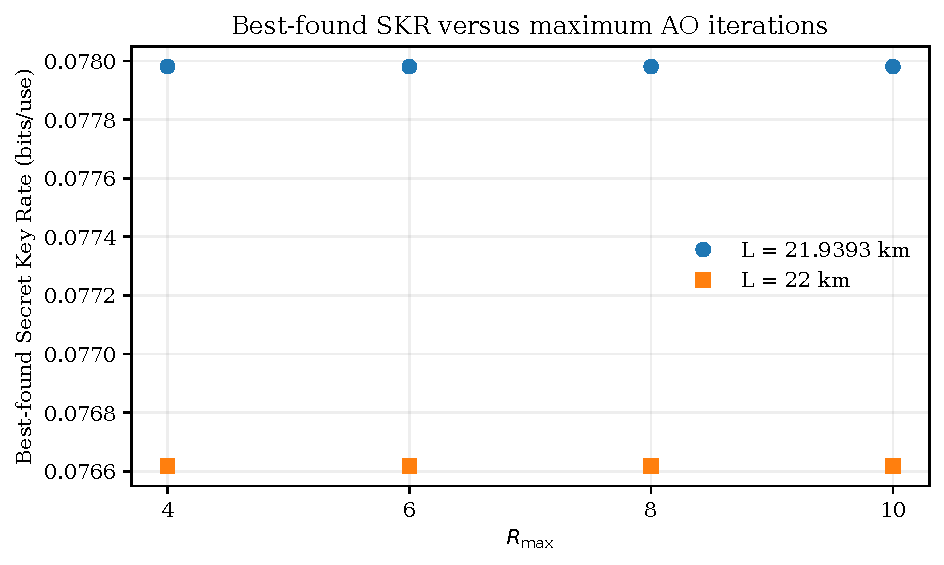
\includegraphics[width=\linewidth]{figures/rmax_sensitivity.pdf}
 \caption{Best-found SKR at the tested caps, with $\epsilon=10^{-8}$.
 Each marker is an actual cache-only AO result. Identical values do not
 imply completed coordinate searches.}
 \label{fig:rmax-sensitivity}
\end{figure}
\begin{figure}[t]
 \centering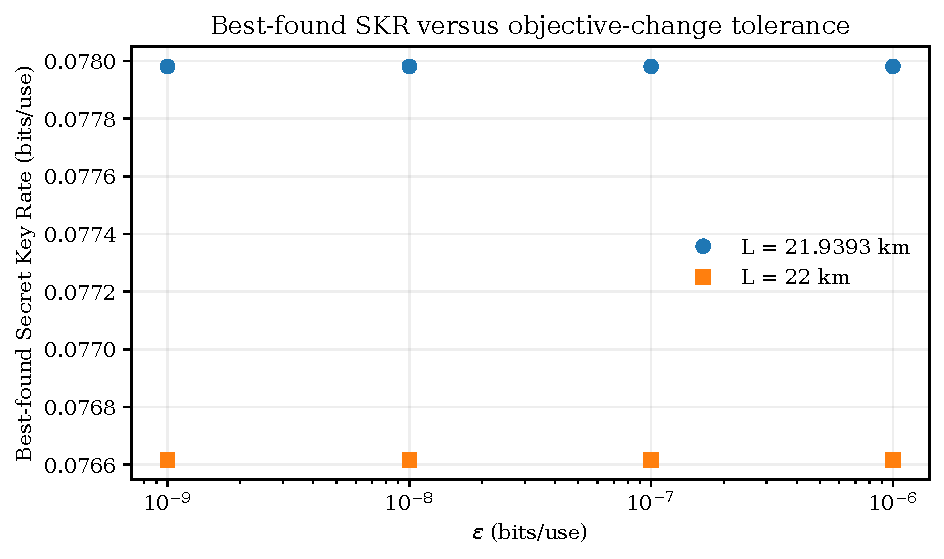
\includegraphics[width=\linewidth]{figures/epsilon_sensitivity.pdf}
 \caption{Best-found SKR at the tested objective-change thresholds, with
 $R_{\max}=6$ and a base-10 logarithmic tolerance axis. The selected SKR
 remains unchanged; the aggregate iteration count decreases at $10^{-6}$.}
 \label{fig:epsilon-sensitivity}
\end{figure}
